% Created 2021-11-11 Thu 22:25
% Intended LaTeX compiler: pdflatex
\documentclass[11pt]{article}
\usepackage[utf8]{inputenc}
\usepackage[T1]{fontenc}
\usepackage{graphicx}
\usepackage{longtable}
\usepackage{wrapfig}
\usepackage{rotating}
\usepackage[normalem]{ulem}
\usepackage{amsmath}
\usepackage{amssymb}
\usepackage{capt-of}
\usepackage{hyperref}
\author{Diogo Garbinato de Fagundes}
\date{\today}
\title{Aula07}
\hypersetup{
 pdfauthor={Diogo Garbinato de Fagundes},
 pdftitle={Aula07},
 pdfkeywords={},
 pdfsubject={},
 pdfcreator={Emacs 27.1 (Org mode 9.6)}, 
 pdflang={English}}
\begin{document}

\maketitle
\tableofcontents


\section{Introdução}
\label{sec:org73b4e7b}

Caro(a) aluno(a),

Essa é a nossa sétima e última aula do Curso de Introdução à Lógica de Programação. Nas aulas anteriores, aprendemos o conceito de algoritmo e sua importância na resolução de problemas do cotidiano. Vimos também as estruturas de entrada e saída de dados e as estruturas de decisão.

Na aula passada, aprendemos o funcionamento das estruturas de repetição em algoritmos. Estudamos formas de identificar situações em que estruturas de repetição devem ser utilizadas e os tipos de estruturas de repetição: ENQUANTO e PARA.

Nesta aula, abordaremos o conceito de modularização em algoritmos. Aprenderemos as vantagens de separar instruções em pequenos blocos de código e como reaproveitar trechos de códigos na elaboração de algoritmos. Vamos à aula!

\textbf{Objetivos}
\begin{itemize}
\item Definir o conceito de modularização de instruções;
\item Identificar vantagens da aplicação de módulos na construção de algoritmos;
\item Compreender a diferença entre Procedimentos e Funções.
\end{itemize}

\section{O que é modularização?}
\label{sec:org46bb898}

\textbf{Objetivos}
\begin{itemize}
\item Compreender o conceito de modularização;
\item Entender a importância da modularização para a organização do algoritmo.
\end{itemize}

Nas aulas passadas, aprendemos diversas estruturas presentes em algoritmos como, por exemplo, estruturas de entrada e saída de dados, estruturas de decisão e repetição. A cada nova estrutura apresentada, um universo de opções para criar algoritmos cada vez mais complexos surgia e, com ele, surgiam também novos problemas.

Um exemplo de problema é a repetição de instruções em um algoritmo.  Durante este tópico, veremos que um algoritmo pode ser escrito de uma maneira mais enxuta, aproveitando trechos de instruções que têm a mesma finalidade.

A modularização surge como uma forma de reaproveitar trechos de códigos que estão se repetindo ou, até mesmo, para separar ideias de um algoritmo para que, na sua leitura, seja mais fácil a compreensão.

Vamos, então, analisar o algoritmo abaixo. Você consegue identificar qual é o trecho que está repetido?

\begin{verbatim}
Variáveis:
    b1, h1, b2, h2 : Inteiro
    a1, a2 : Decimal
Início
    b1 = 10
    h1 = 2
    b2 = 14
    h2 = 4
    a1 = (b1*h1)/2
    a2 = (b2*h2)/2
    se a1 > a2 então
         saída(“Triângulo 1 é maior”)
    senão
         saída(“Triângulo 2 é maior ou igual”)
    fim_se
Fim
\end{verbatim}

Se você disse “a1 = (b1*h1)/2” e “a2 = (b2*h2)/2“, você acertou. Veja que apesar das variáveis serem diferentes (b1 é diferente de b2 e h1 é diferente de h2), a operação (multiplicar e depois dividir) é a mesma.

Você consegue descobrir o que a operação “a1 = (b1*h1)/2” faz? Ela calcula a área de um triângulo dada uma base “b1” e uma altura “h1”. E se, durante o algoritmo, precisássemos fazer outra operação para calcular a área de outro triângulo? Uma boa solução seria modularizar essa operação. Vamos analisar um algoritmo um pouco mais complexo para entender melhor o conceito de modularização?

Analise o algoritmo 2 e responda: quais são os valores das variáveis ehBissexto1 e ehBissexto2 no final da execução do algoritmo?

\begin{verbatim}
Variáveis:
    a1, a2 : Inteiro
    ehBissexto1, ehBissexto2 : Booleano
Início
    a1 = 1988
    a2 = 2000
    ehBissexto1 = falso
    ehBissexto2 = falso
    se a1 % 400 == 0 então
         ehBissexto1 = verdadeiro
    fim_se
    se a2 % 400 == 0 então
         ehBissexto2 = verdadeiro
    fim_se
    se a2 % 4 == 0 && a2 % 100 != 0 então
         ehBissexto2 = verdadeiro
    senão
         ehBissexto2 = falso
    fim_se
Fim
\end{verbatim}

Para analisarmos o algoritmo 2, precisamos, antes, conhecer a função do símbolo “\%”. Esse símbolo, em um algoritmo, representa a operação “resto da divisão”. Por exemplo: o resto da divisão de 10 por 2 é 0 e o resto da divisão de 3 por 2 é 1. Veja mais exemplos:

4 \% 2 = 0
14 \% 5 = 4
5 \% 3 = 2
21 \% 3 = 0
Vamos fixar nossos conhecimentos com o novo operador?

Analise as operações abaixo e informe a resposta de cada item. Exemplo: “3 \% 2 = 1”

4 \% 2 = ?
135 \% 3 = ?
3 \%  4 = ?
10 \% 9 = ?

O algoritmo 2 tem como finalidade verificar se os anos 1988 e 2000 são bissextos. Conseguiu identificar qual é o trecho do código que tem a mesma operação? O trecho que possui a mesma operação é responsável por verificar se, dado um ano (variável “a1” ou “a2”), ele é ou não bissexto (o resultado dessa operação é guardada na variável “ehBissexto1” ou “ehBissexto2”). Veja com mais detalhes os trechos na figura 1:

\begin{verbatim}
Figura 1 - Trecho de código repetido no algoritmo 2
se a1 % 400 == 0 então
ehBissexto1 = verdadeiro
fim_se
se a1 % 4 == 0 && a1 % 100 != 0 então
ehbissexto1 = verdadeiro
senão
ehbissexto1 = falso
fim_se
\end{verbatim}

\begin{verbatim}
se a2 % 400 == 0 então
  ehBissexto2 = verdadeiro
fim_se
se a2 % 4 == 0 && a2 % 100 != 0 então
  ehbissexto2 = verdadeiro
senão
  ehbissexto2 = falso
fim_se
\end{verbatim}

\begin{quote}
Um ano é dito bissexto quando é acrescentado um dia no mês de fevereiro, o que faz com que o ano tenha 366 dias, um dia a mais do que os anos normais de 365 dias. Essa adição ocorre a cada quatro anos (exceto anos múltiplos de 100 que não são múltiplos de 400). Essa operação é realizada com o objetivo de manter o calendário anual ajustado com a translação da Terra e com os eventos sazonais relacionados às estações do ano
\end{quote}
Veja que, conforme a figura 1, precisamos de oito linhas de instruções para verificar se um ano é bissexto. No nosso exemplo, verificamos apenas se dois anos são ou não bissextos (1988 e 2000). E se quiséssemos verificar dez anos? Consegue imaginar a quantidade de instruções que irão se repetir e que fazem basicamente a mesma coisa?

E se pudéssemos separar essas instruções que fazem a mesma coisa em um trecho do algoritmo e ficássemos “chamando” toda vez que precisássemos reutilizar essas instruções?

Modularizar um algoritmo é separar partes das instruções em blocos que depois podem ou não ser reutilizados em outras partes do algoritmo, fazendo com que sua manutenção seja mais fácil e que haja uma simplificação maior no algoritmo.

A modularização é parte importante na construção de algoritmos, principalmente em empresas que possuam mais de um desenvolvedor trabalhando com os mesmos algoritmos.

Um desenvolvedor pode, por exemplo, estar trabalhando em um módulo de contas a receber e um outro pode estar trabalhando em um módulo de vendas. Perceba que cada módulo tem uma finalidade específica e essa é outra boa forma de utilização de módulos: separar por responsabilidades (ou por funções) a sua utilização.

\begin{center}


\includegraphics[width=.9\linewidth]{figura02.png}

\caption{Figura 2 - Exemplos de Módulos em Sistemas Empresariais}

\end{center}



Analisando a figura 2 é possível perceber a divisão de responsabilidades em um algoritmo onde cada módulo possui sua responsabilidade bem definida. Por exemplo, se precisamos descobrir se o produto A ainda tem estoque, acessamos o módulo “Controle de Estoque” ou, se precisamos saber se o cliente B possui algum pagamento pendente, acessamos o módulo “Contas a Receber”.

Com isso, ganhamos em manutenção (podemos ir direto a um módulo para fazer a correção no algoritmo) e reutilização de código (podemos utilizar instruções já definidas em outros módulos).

\begin{quote}
Sobre modularização em algoritmos, selecione o item verdadeiro.
\begin{enumerate}
\item Modularizar um algoritmo é identificar estruturas de repetição no código e reutilizar em outros lugares.
\item O único objetivo de modularizar é diminuir a quantidade de instruções no algoritmo.
\item Modularização de algoritmo, além de reutilizar trechos de códigos, facilita a manutenção por outros desenvolvedores.
\item Apenas sistemas complexos podem ser modularizados.
\end{enumerate}
Fim
\end{quote}

Atenção! O uso de módulos em algoritmos faz com que o fluxo de execução do algoritmo seja desviado para dentro do módulo e depois retorne para o fluxo principal. Vamos analisar a figura 3 :

\begin{center}
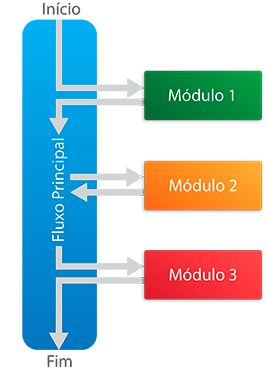
\includegraphics[width=.3\linewidth]{figura03.png}


\caption{Figura 3 - Fluxo de execução de um Módulo}
\end{center}


O processador sempre vai começar a executar um algoritmo pelo fluxo principal, executando instrução após instrução, até encontrar um módulo. Quando isso acontecer, ele vai \textbf{parar} a execução das instruções no fluxo principal e executar todas as instruções que estão dentro do módulo. Quando o processador terminar de executar o módulo, ele volta para o ponto onde parou (antes de entrar no módulo) e continua a sua execução.

Para ficar mais claro, na figura 3, o processador inicia executando as instruções que estão no fluxo principal e pausa a execução para executar o módulo 1. Ao terminar o módulo 1 (tendo executado todas as instruções), volta a executar instruções no fluxo principal até encontrar o módulo 2. Executa as instruções do módulo 2 e volta para o fluxo principal para executar as outras instruções. Por fim, executa as instruções contidas no módulo 3 e, ao final, executa as últimas instruções do fluxo principal antes de encerrar.

Observe o vídeo 1 e entenda melhor o fluxo de execução de um módulo a partir do fluxo principal:
\url{video01.mp4}

É interessante notar que um módulo também pode chamar \textbf{um ou mais} módulos, inclusive, \textbf{ele mesmo}. Observe a figura 4.

Veja que o processador começa executando o fluxo principal e pausa porque encontrou uma chamada ao módulo 1. Ele entra no módulo 1 para executar as instruções e pausa também, pois, lá dentro tem uma chamada ao módulo 2. Ele entra no módulo 2, executa todas as instruções e volta para o módulo 1 na posição de onde parou. Termina de executar o módulo 1 e volta para o fluxo principal do algoritmo, executando o restante das instruções antes de finalizar o fluxo.

\begin{center}

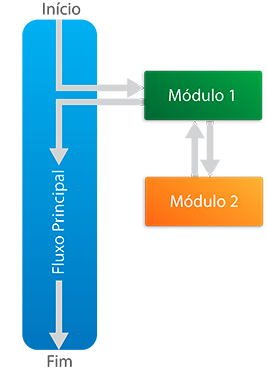
\includegraphics[width=.3\linewidth]{figura04.png}

\caption{Figura 4 - Módulo chamando outro Módulo no mesmo algoritmo}

\end{center}


Observe o vídeo 2 e entenda melhor o processo de execução de um módulo a partir de outro módulo:
\url{video02.mp4}

Nesse tópico, aprendemos o quanto é importante a modularização do algoritmo na reutilização de instruções e manutenção. Além disso, utilizando alguns exemplos, aprendemos a identificar situações onde a modularização pode ser aplicada.

No próximo tópico, conheceremos os tipos de modularização, suas particularidades e a forma de utilização em algoritmos.

\section{Procedimentos x Funções}
\label{sec:org20662f5}
\textbf{Objetivos}
\begin{itemize}
\item Compreender a diferença entre procedimentos e funções;
\item Identificar os casos de aplicação de procedimentos e funções em algoritmos.
\end{itemize}

No tópico anterior, entendemos a importância da utilização de módulos para criar algoritmos cada vez mais reutilizáveis e de fácil manutenção.

Existem dois tipos de módulos em algoritmos. São eles:

\begin{itemize}
\item Procedimentos – módulos que recebem uma lista de parâmetros e não retornam um valor. Por exemplo, um procedimento de enviar e-mail não precisa retornar nada.
\item Funções – módulos que recebem uma lista de parâmetros e, obrigatoriamente, retornam algum valor. Por exemplo, uma função para calcular a raiz quadrada de um número retorna o valor da raiz quadrada.
\end{itemize}

Para cada um dos tipos de módulo (função e procedimento) existe uma regra de formação específica. Vamos estudar cada tipo de módulo separado para compreender melhor o seu funcionamento e sua estrutura.

Antes de entrarmos nas definições de procedimentos e funções, precisamos estudar um pouco sobre Parâmetros. O que são parâmetros e como utilizar? 

\subsection{Parâmetros}
\label{sec:orge016c20}

Parâmetros são valores que passamos para os módulos antes de executá-los. Por exemplo, vamos imaginar um módulo que tem como objetivo verificar se um dado ano é bissexto ou não. Um possível parâmetro para esse módulo seria o ano. Precisaríamos informar ao módulo o ano para que ele verifique se é bissexto ou não.

Vamos a outro exemplo: imagine, agora, um módulo responsável por calcular a área de um triângulo. Quais informações o módulo precisa para calcular a área de um triângulo? Acertou quem disse o valor da “base” e o valor da “altura” do triângulo. Sem essas informações, o módulo de calcular a área do triângulo não iria funcionar.

Os \textbf{Procedimentos} e \textbf{Funções} têm em comum os parâmetros que devem ser informados na construção do módulo. Um detalhe importante é que os parâmetros não são obrigatórios em módulos, ou seja, podemos ter procedimentos e funções sem nenhum parâmetro.

O módulo de calcular a área de um triângulo precisa ter dois parâmetros para executar, são eles: base e altura do triângulo. Já o módulo de calcular a raiz de um número precisa ter como parâmetro o número que se deseja calcular a raiz, enquanto o módulo responsável por exibir na tela do menu de um sistema não precisa ter nenhum parâmetro.

Os parâmetros nada mais são do que variáveis que deverão ser preenchidas sempre que você precisar chamar um procedimento ou função. Veja na figura 5 a regra de formação de parâmetros:

(<nome\textsubscript{da}\textsubscript{variavel}> : <tipo\textsubscript{da}\textsubscript{variavel}>)
    figura 5 - Regra de formação de parâmetros

Para criar parâmetros no módulo, você precisa definir o nome das variáveis seguidas pelo tipo (Inteiro, Decimal, Texto, Caractere, Booleano).

Exemplos de parâmetros:

\begin{itemize}
\item (a,b: Inteiro)
\item (a: Inteiro, b: Decimal)
\item (a: Booleano,b:Inteiro,c:Texto)
\item (a,b:Decimal, c,d: Decimal)
\end{itemize}

Uma vez definidos os parâmetros para um módulo, você precisará sempre informar todos os valores para cada um, pois, sem isso, o algoritmo não irá funcionar. Por exemplo, se você criou um módulo com três parâmetros (a,b,c) e precisa chamá-lo, você precisa então informar os valores de cada uma das variáveis.

Nas próximas seções, exemplos de módulos com parâmetros serão utilizados para fixar melhor esses conceitos.

\begin{quote}
Parâmetros são variáveis que somente existem durante a execução de um procedimento ou função. Sempre que um procedimento ou função terminar a sua execução, os parâmetros serão eliminados da memória pelo processador.
\end{quote}

\subsection{Procedimentos}
\label{sec:org994801f}
Procedimentos são módulos responsáveis por executar instruções e que não retornam nenhum valor no final da sua execução. A figura 6 mostra a regra de formação de um procedimento:

\begin{verbatim}
*procedimento* <nome_do_procedimento> ( <lista_de_parametros> )
Variáveis:
<lista_de_variaveis>
*Inicio*:
...
*fim_procedimento*
\end{verbatim}
Figura 6 - Regra de formação de um Procedimento

Para definir um módulo do tipo \textbf{procedimento}, é preciso iniciar o bloco com a palavra-chave “procedimento” e, logo em seguida, definir o nome para o seu procedimento. Será através dele que você irá fazer a chamada no algoritmo para que suas instruções sejam executadas. Logo em seguida, você deve definir os parâmetros para o seu procedimento.

\begin{quote}
A lista de parâmetros é opcional, ou seja, o módulo não precisa necessariamente ter parâmetros, mas se tiver algum, todos devem ser preenchidos quando forem chamados.
\end{quote}
As instruções que deverão ser executadas no procedimento devem estar escritas depois da palavra-chave “Inicio” e as variáveis utilizadas, depois da palavra-chave “Variáveis”. Para finalizar o módulo, você precisa apenas fechar o bloco com a palavra-chave “fim\textsubscript{procedimento}”.

Vamos analisar um algoritmo para tentarmos fixar os conhecimentos acerca de procedimentos.

\begin{verbatim}
Algoritmo 3: Exibir na tela Olá Mundo
1 Variáveis:
2 procedimento exibirFrase()
3 Variáveis
4 Inicio
5    saida(“Olá Mundo”)
6 fim_procedimento
7 Início
8 exibirFrase()
Fim
\end{verbatim}

O algoritmo 3 exibe na tela a frase “Olá Mundo”. Veja que a frase foi colocada dentro do procedimento “exibirFrase” e quando o procedimento é chamado, a frase aparece na tela.

Iniciamos nosso algoritmo definindo que ele terá um módulo do tipo procedimento, chamado “exibirFrase”, que será responsável por exibir na tela a mensagem “Olá Mundo” como pode ser visto depois da palavra-chave “Inicio” do procedimento.

Uma vez definido um módulo, ele precisa ser necessariamente chamado. Se você definiu um módulo e não o chamou, ele não vai ser executado. E como é que nós chamamos um módulo? Simples, basta utilizar o nome que você definiu no módulo e passar os valores como parâmetros (caso ele utilize parâmetros). No exemplo do algoritmo 3, criamos um módulo na linha 2 (que não tem nenhum parâmetro) e o chamamos na linha 8.

Vamos analisar agora o algoritmo 4. Ele possui um procedimento que recebe como parâmetro dois números, executa a operação de soma, guardando o resultado na variável “c”, e exibe na tela do usuário o resultado de “c”. O procedimento possui dois parâmetros, a e b, do tipo inteiro.

\begin{verbatim}
Algoritmo 4: Soma dois  Números
1 Variáveis:
2 procedimento somarNumeros(a,b:Inteiro)
3 Variáveis
4    c : Inteiro
5 Inicio
6    c = a + b
7    saida(c)
8 fim_procedimento
9 Início
10  somarNumeros(2,3)
11  somarNumeros(5,6)
Fim
\end{verbatim}

Na linha 10 do algoritmo 4, chamamos o procedimento passando por parâmetros dois números: o número 2 e o número 3. Como o procedimento tem dois parâmetros a e b, o processador entende que você quer atribuir o valor 2 à variável a e o valor 3 à variável b.  O processador executa o procedimento “somarNumeros” que corresponde a somar a e b, e coloca o resultado na variável c. No final, exibe, na tela, o valor da variável c.

No algoritmo 4 temos duas chamadas ao procedimento “somarNumeros”. A primeira chamada, passando por parâmetro o número 2 e 3 e na outra passamos por parâmetro o número 5 e 6.

Analise o algoritmo 4 e responda: no final da execução, qual será a saída do algoritmo? Ele vai exibir na tela os números “5 e 11”. O 5 corresponde à chamada do procedimento “somarNumeros(2,3)” e o 11 corresponde à chamada do procedimento “somarNumeros(5,6)”.

Quiz - A partir do que vimos sobre procedimentos, analise o algoritmo abaixo e informe a saída dele.

Variáveis:
  a, b: Inteiro
  procedimento areaDoQuadrado (l: Inteiro)
  Variáveis
    c: Inteiro
  Inicio
    c = l * l
    se c < 10 então
         saida(“Área menor do que 10”)
    então
         saida(“Área maior ou igual a 10”)
    fim\textsubscript{se}
  fim\textsubscript{procedimento}
Início
  areaDoQuadrado(3)
  areaDoQuadrado(5)
Fim

\begin{enumerate}
\item areaDoQuadrado(3) | \emph{Área menor do que 10} | \emph{Área maior ou igual a 10} |
\item areaDoQuadrado(5) | \emph{Área menor do que 10} | \emph{Área maior ou igual a 10} |
\end{enumerate}

\subsection{Funções}
\label{sec:orga2d71d3}
Funções são módulos responsáveis por executar instruções e que, obrigatoriamente, retornam algum valor no final da sua execução. A figura 7 mostra a regra de formação de uma função:

\begin{verbatim}
funcao <nome_da_funcao> ( <lista_de_parametros> ) : <tipo_de_retorno>
Variaveis:
  <lista_de_variaveis>
Inicio:
  ...
  retorno <valor_retorno>
fim_funcao
\end{verbatim}

\caption{Figura 7 - Regra de formação de uma Função}



A forma de definir uma \textbf{função} é muito parecida com a forma de definir um procedimento. Iniciamos esse tipo de módulo com a palavra-chave “funcao” seguida pelo nome da função que iremos chamar. Depois, passamos a lista de parâmetros que a função utilizará, seguida pelo tipo \textbf{do retorno da função}.

Como uma função obrigatoriamente retorna algum valor, precisamos definir na função qual o tipo do retorno que ela possui (Inteiro, Decimal, Booleano, Caractere ou Texto). Por exemplo, quando somamos dois números Inteiros, o resultado é outro número Inteiro. Um possível retorno para a função que soma dois números inteiros seria \textbf{Inteiro}.

Todas as instruções que serão executadas pela função devem iniciar depois da palavra-chave “Inicio”. Por fim, o bloco da função é finalizado com a palavra-chave “fim\textsubscript{funcao}”.

Toda função deve ter a instrução \textbf{“retorne”} na sua execução. É através dessa instrução que a função irá retornar um valor para o fluxo que a chamou. Por exemplo: se o fluxo principal chamou a função, ela irá retornar o valor descrito na instrução para o fluxo principal.

Um detalhe muito importante: sempre que o processador encontrar a instrução “retorne” dentro de uma função, ele vai \textbf{encerrar} a sua execução e retornar o valor encontrado para o fluxo que o chamou. Veja, na figura 8 , que o comando “c++” \textbf{não} será executado porque, antes dele, o processador encontrou uma instrução “retorne c”.

\begin{verbatim}
funcao funcA(a: Inteiro): Inteiro
Variáveis
  c : Inteiro
Inicio
  c = 2 + a
  retorne c
  c++;
fim_funcao
\end{verbatim}
Figura 8 – Exemplo de instrução inalcançável após cláusula ‘retorne’

Vamos analisar o algoritmo 5 a seguir. Ele é responsável por verificar se um dado número é par ou ímpar. Para fazer essa verificação, utilizaremos novamente o operador “\%” descrito no tópico 1 desta aula. Um número é par se o resto da divisão dele por 2 for igual a 0, caso contrário, ele é ímpar.

\begin{verbatim}
Variáveis:
    r: Inteiro
    funcao restoDaDivisao(a: inteiro): Inteiro
    Variáveis
    c: Inteiro
    Inicio
        c = a % 2
        retorne c
    fim_funcao
Início
    r = restoDaDivisao(10)

    se r == 0 então
        saida("par");
    senão
        saida("impar")
    fim_se
Fim
\end{verbatim}
Algoritmo 5: Resto da divisão

Na linha 11 do algoritmo 5, vemos uma chamada à função “restoDaDivisao”, passando por parâmetro o número 10. Nesse momento, o fluxo é interrompido para a execução da função. O valor 10 é atribuído à variável a, presente nos parâmetros, e a instrução “c = a \% 2” é executada, guardando, assim, o valor 0 na variável c. Por fim, vemos que a variável c é retornada na linha 8 para o ponto onde a função foi chamada.

Lembram que o fluxo de execução tinha parado na linha 11? Qual foi o retorno da função? O valor retornado da função foi 0. Esse valor será atribuído ou guardado na variável r devido ao operador “=”.

Por fim, como a variável r guarda o valor 0, a condição “r == 0” é verdadeira exibindo, assim, na tela a saída “par”.

Toda \textbf{função} deve obrigatoriamente ter a instrução “retorne” seguida de um valor ou variável para funcionar. Lembre-se que uma função \uline{sempre} retorna algum valor e é essa a instrução que determina o que será retornado.

Vamos analisar outro exemplo. O algoritmo 6 é responsável por calcular a média de um aluno e verificar se o mesmo passou na disciplina.

\begin{verbatim}
1 Variáveis:
2 nota1,nota2,n: Decimal
3 funcao mediaDoAluno(n1,n2: Decimal): Decimal
4 Variáveis
5   media : Decimal
6 Inicio
7   media = (n1 + n2)/2
8   retorne media
9 fim_funcao
10
11 procedimento passouNaDisciplina(m: Decimal)
12  Variáveis
13  Inicio
14    se m >= 7 então
15      saida(“Aprovado”);
16    senão
17      saida(“Reprovado”)
18    fim_se
19 fim_procedimento
20 Início
21  nota1 = 6
22  nota2 = 7
23  n = mediaDoAluno(nota1,nota2)
24  passouNaDisciplina(n);
25 Fim
\end{verbatim}
Algoritmo 6: Passou na disciplina

Conseguiram identificar que o algoritmo 6 possui dois módulos? Quais são eles? O primeiro é a \textbf{função} chamada “mediaDoAluno” que, dados dois parâmetros, retorna a média e o \textbf{procedimento} chamado “passouNaDisciplina”, que escreve na tela se o aluno passou ou não na disciplina.

Veja que, na linha 23, chamamos a função “mediaDoAluno” passando como parâmetro as variáveis “nota1” e “nota2”. O valor dessas variáveis é atribuído aos parâmetros “n1” e “n2” respectivamente.

A função calcula a média dos números guardando o valor final na variável “media”. Por fim, a função retorna o valor guardado na variável “media” para o ponto onde ela foi chamada, no caso, na linha 23.

O valor retornado é, então, guardado ou atribuído à variável n que, logo em seguida, é passada por parâmetro para o procedimento “passouNaDisciplina”, que terá como objetivo exibir na tela a frase de “Aprovado” ou “Reprovado”.

De posse dessas informações, qual será a saída do algoritmo para os valores em questão? Se você respondeu “Reprovado”, você acertou.

Como uma \textbf{função} retorna um valor, é comum a sua chamada vir logo após um operador de atribuição “=” pois queremos guardar o valor retornado por ela em uma variável para depois utilizarmos. O mesmo não é válido para procedimentos pois eles não retornam \uline{valor algum} e, por isso, não podem atribuir a uma variável.

\begin{verbatim}
Variáveis:
  m: Inteiro
  funcao funcA(a,b: Inteiro): inteiro
  Variáveis
    c: Inteiro
  Inicio
    c = a - b
    retorne c
  fim_funcao

  funcao funcB(d,e: Inteiro): inteiro
  Variáveis
    f,g,h: Inteiro
  Inicio
    f = funcA(10,d)
    g = funcA(5,e)
    h = f + g
    retorne h
  fim_funcao
Início
  m = funcB(3,2)
Fim
\end{verbatim}

Analise o algoritmo acima e informe o valor da variável m no final da execução: |         |

Para cada item, defina qual tipo de módulo é mais recomendado (Procedimento ou Função) utilizar.

\begin{enumerate}
\item Exibir um menu do sistema.
Procedimento/Função

\item Exibir uma mensagem de erro do sistema.
Procedimento/Função

\item Calcular a raiz quadrada de um número.
Procedimento/Função

\item Calcular o logaritmo de um número.
Procedimento/Função
\end{enumerate}

Funções e Procedimentos podem ter o mesmo nome das variáveis. Como o processador consegue diferenciar uma variável de uma função ou procedimento? Ele faz isso na forma de chamar a função. Lembra que precisamos passar parâmetros para um módulo? É através dos parâmetros que o processador sabe que queremos executar um módulo e não uma variável.

Um algoritmo também pode ter várias funções com o mesmo nome, mas com \textbf{parâmetros e retornos diferentes}. Por exemplo:

\begin{enumerate}
\item funcao funcA(a: Inteiro): Inteiro
\item funcao funcA(a: Inteiro, b: Decimal): Inteiro
Figura 9 - Funções com mesmo nome
\end{enumerate}

Como o processador sabe diferenciar funções que possuem o mesmo nome? O processador vai analisar os parâmetros passados quando a função ou procedimento for chamado. De acordo com a figura 9, se a função for chamada através da instrução “funcA(2)”, a função 1 será chamada. Caso a função seja chamada usando “funcA(2,3)”, a função 2 será chamada.

Para utilizar uma função ou procedimento, você precisa necessariamente declarar antes de usar. Por exemplo, para utilizar a função “aplicarDesconto”, você precisa declarar o módulo na seção “Variáveis” do algoritmo. Vamos, agora, aprender a declarar e chamar uma função ou procedimento.

Observe a figura 10 e veja como fazer a declaração e a chamada de uma função:

\begin{center}

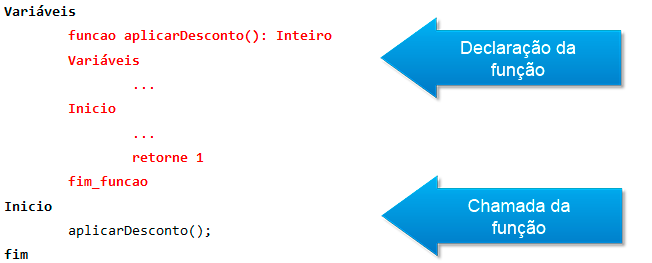
\includegraphics[width=.9\linewidth]{figura11.png}

\caption{Figura 10 – Declarar e chamar uma função}

\end{center}


Veja na figura 11 como fazer a declaração e a chamada de um procedimento:

\begin{center}

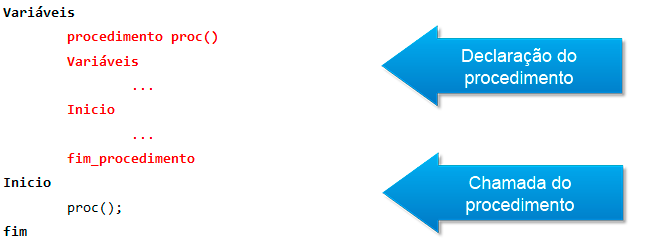
\includegraphics[width=.9\linewidth]{figura12.png}

\caption{Figura 11 – Declarar e chamar um procedimento}

\end{center}

Concluímos a nossa sétima e última aula do Curso de Introdução à Lógica de Programação. Aprendemos sobre modularização em algoritmos e como é importante o seu papel na construção de algoritmos cada vez mais complexos e que, ao mesmo tempo, tenha uma grande capacidade de reutilização de código. Além disso, aprendemos que existem dois tipos de módulos: \textbf{procedimentos} (módulos que não retornam nenhum valor) e \textbf{funções} (módulo que retorna algum valor obrigatoriamente). Aprendemos a construir e identificar esses módulos além de utilizar em vários algoritmos.

Chegamos também ao fim do nosso curso de Lógica. Aqui, abordamos a lógica de programação desde os componentes de um computador até o seu funcionamento através de algoritmos. Passamos por diversos assuntos onde, dentre eles, tipos de dados, variáveis, estruturas de decisão e repetição. Com isso, temos todo o conhecimento necessário para avançar nos próximos cursos e aprender um pouco mais sobre como desenvolver algoritmos capazes de resolver diversos problemas do dia a dia.

Fim
\end{document}
